\documentclass[
11pt,%
tightenlines,%
twoside,%
onecolumn,%
nofloats,%
nobibnotes,%
nofootinbib,%
superscriptaddress,%
noshowpacs,%
centertags]%
{revtex4}
\usepackage{ljm}
\usepackage{listings}
\usepackage{amsmath}

\lstset{
language=C++,
basewidth=0.5em,
xleftmargin=45pt,
xrightmargin=45pt,
basicstyle=\small\ttfamily,
keywordstyle=\bfseries\underbar,
numbers=left,
numberstyle=\tiny,
stepnumber=1,
numbersep=10pt,
showspaces=false,
showstringspaces=false,
showtabs=false,
frame=trBL,
tabsize=2,
captionpos=t,
breaklines=true,
breakatwhitespace=false,
escapeinside={\%*}{*)}
}

\begin{document}

\titlerunning{Scaling of supercomputer calculations}
\authorrunning{Shabanov et al.}

\title{Исследование эффективности масштабирования суперкомпьютерных вычислений на неструктурированных поверхностных расчетных сетках}

\author{\firstname{B.~M.}~\surname{Shabanov}}
\email[E-mail: ]{shabanov@jscc.com}
\affiliation{Joint Supercomputer Center of the Russian Academy of Sciences -- branch of Scientific Research Institute of System Analysis of the Russian Academy of Sciences, Leninsky prospect 32a, Moscow, 119334, Russia}

\author{\firstname{A.~A.}~\surname{Rybakov}}
\email[E-mail: ]{rybakov.aax@gmail.com}
\affiliation{Joint Supercomputer Center of the Russian Academy of Sciences -- branch of Scientific Research Institute of System Analysis of the Russian Academy of Sciences, Leninsky prospect 32a, Moscow, 119334, Russia}

\author{\firstname{S.~S.}~\surname{Shumilin}}
\email[E-mail: ]{shumilin@jscc.com}
\affiliation{Joint Supercomputer Center of the Russian Academy of Sciences -- branch of Scientific Research Institute of System Analysis of the Russian Academy of Sciences, Leninsky prospect 32a, Moscow, 119334, Russia}

\author{\firstname{M.~Yu.}~\surname{Vorobyov}}
\email[E-mail: ]{nordmike@jscc.com}
\affiliation{Joint Supercomputer Center of the Russian Academy of Sciences -- branch of Scientific Research Institute of System Analysis of the Russian Academy of Sciences, Leninsky prospect 32a, Moscow, 119334, Russia}

\firstcollaboration{(Submitted by A.~M.~Elizarov)} % Add if you know submitter.
%\lastcollaboration{ }

\received{TODO}

\begin{abstract}
При решении комплексных задач численного моделирования используются расчетные сетки, содержащие десятки и сотни миллионов ячеек.
Постепенно потребности в вычислительных ресурсах возрастают, и расчетные задачи в современной постановке переходят черту в миллиард ячеек.
Локальные вычислительные станции не способны справиться с такими объемами данных и вычислений.
Для выполнения вычислений такого объема требуется использование суперкомпьютерных кластеров, состоящих из многих вычислительных узлов, связанных между собой высокоскоростной коммуникационной сетью.
При этом необходимо выполнять декомпозицию расчетной сетки на отдельные домены, чтобы обеспечить ее параллельную обработку сразу на всех узлах кластера.
Эти домены распределяются по вычислительным узлам суперкомпьютера и обрабатываются независимо друг от друга.
Для синхронизации вычислений после каждой итерации обработки ячеек производятся обмены данными на границах между соседними соприкасающимися доменами.
Для эффективности выполнения вычислений и масштабирования их на большое количество вычислительных узлов требуется разработка эффективных алгоритмов декомпозиции расчетных сеток, порождающих множество доменов с накладываемыми на них требованиями по количеству ячеек, равномерности распределения ячеек по доменам, связности доменов и размеру границ между ними.
При этом теоретические показатели эффективности декомпозиции расчетной сетки не гарантируют эффективного выполнения реальной задачи на суперкомпьютере.
В данной статье в качестве объекта исследования рассматривается неструктурированная поверхностная сетка, используемая для расчета процессов взаимодействия объемного тела с окружающей средой.
Для сетки такого вида рассматривается иерархический алгоритм декомпозиции с выбором оптимального критерия разбиения на домены.
С использованием данного алгоритма декомпозиции проводятся суперкомпьютерные расчеты на вычислительных ресурсах МСЦ РАН с целью измерения практических показателей масштабируемости высоконагруженных приложений.
\end{abstract}

\subclass{65Y05,65Y20,49M27} % Enter 2010 Mathematics Subject Classification.

\keywords{суперкомпьютер, поверхностная неструктурированная расчетная сетка, декомпозиция, домен, высокопроизводительные вычисления, масштабирование вычислений}

\maketitle

\section{Introduction}

Современные расчетные приложения крайне требовательны к вычислительным ресурсам.
Для больших задач не представляется возможным выполнение их на отдельно взятом вычислителе (одном микропроцессоре или одном сервере) за приемлемое время.
Возникает потребность использовать для вычислений суперкомпьютерные кластеры, состоящие из многих вычислительных узлов.
Для того, чтобы выполнить задачу на суперкомпьютере, необходимо разделить ее расчетную область на отдельные подобласти, называемые доменами, и обрабатывать эти домены параллельно и независимо друг от друга.
Для повышения эффективности суперкомпьютерных приложений внутри вычислительного узла применяются различные методы подготовки данных и распараллеливания исполнения для систем с общей памятью, а также низкоуровневые оптимизации программного кода, такие как векторизация, позволяющие существенно повысить скорость выполнения приложений.
Конечно, на границах соприкосновения доменов возникает необходимость синхронизации вычислений, что достигается путем обмена данными (например, с использованием MPI).
Таким образом, выполнение суперкомпьютерных расчетов состоит из двух чередующихся шагов: параллельная обработка ячеек расчетной области и обмен данными на границах соприкосновения доменов, обрабатываемых различными процессами.
Эффективность выполнения суперкомпьютерных приложений существенным образом зависит от качества декомпозиции расчетной сетки и ее распределения между разными вычислительными узлами.

Данная статья посвящена задаче декомпозиции поверхностной неструктурированной расчетной сетки для распределения между узлами гомогенного суперкомпьютерного кластера (то есть кластера, состоящего из одинаковых вычислительных узлов) для повышения эффективности масштабирования вычислений.
Пусть дана поверхностная сетка, состоящая из $S$ расчетных ячеек, пусть также суперкомпьютер состоит из $n$ вычислительных узлов с одинаковыми характеристиками.
Также будем считать, что скорость обмена данными между любыми двумя вычислительными узлами одинакова для всех узлов.
Распространение задачи распределения вычислительной нагрузки на гетерогенный вычислительный кластер достигается путем ввода весовых коэффициентов для вычислительных узлов и для каналов обмена данными, как это описано в.
Если представить скорость обработки расчетных ячеек на одном вычислительном узле как $a^{-1}$, то время выполнения одной итерации расчетов на одном вычислительном узле будет равно $T_1 = aS$.
Пусть теперь расчетная область разбита на $n$ доменов, содержащих по $S_i$ ячеек ($i=1,n$).
Обозначим через $L_{ij}$ количество ребер, составляющих границу между доменами $S_i$ и $S_j$.
Будем считать, что каждый домен обрабатывается на своем вычислительном узле.
Таким образом, все домены обрабатываются параллельно, и время обработки всех ячеек определяется временем обработки самого крупного домена.
Кроме обработки всех расчетных ячеек после проведения итерации расчета необходимо выполнить обмен данными между всеми парами доменов по всем границам между ними.
Пусть скорость передачи данных между узлами определяется величиной $b^{-1}$, и все обмены выполняются параллельно, тогда время выполнения всех обменов определяется временем обмена данными через самую длинную границу.
Исходя из этого, можно определить суммарное время выполнения одной итерации расчета при выполнении на $n$ вычислительных узлах:

\begin{equation}
T_n = a \max_{i = 1,n}{S_i} + b \max_{i,j=1,n}{L_{ij}}
\end{equation}

Критерием оптимизации декомпозиции расчетной сетки является сокращение времени выполнения расчетов, то есть величины $T_n$.
Время выполнения расчетов напрямую зависит от размера самого крупного домена, однако мы будем рассматривать не абсолютный размер домена, а его отклонение от теоретического оптимального значения.
Очевидно, что в идеальном случае при декомпозиции все домены должны иметь размер $\frac{S}{n}$, а относительное отклонение от идеального размера в процентах можно вычислить по формуле

\begin{equation}
D = 100 \% \left( \frac{n}{S} \max_{i=1,n}{S_i} - 1 \right)
\end{equation}

Вторым важным критерием качества выполненной декомпозиции является наибольшее значение длины границы между парами доменов.
В данном случае можно использовать абсолютную характеристику, так как длину границы предсказать довольно сложно, и у нее вообще говоря нет теоретического минимума (в зависимости от геометрии рассматриваемой сетки теоретически длина границы между доменами может быть нулевой).
То есть в качестве критерия сравнения различных методов декомпозиции сетки будем использовать следующую величину:

\begin{equation}
L = \max_{i,j=1,n}{L_{ij}}
\end{equation}

Несмотря на то, что в наших предположениях все обмены данными между доменами выполняются одновременно, общий объем всех обменов существенно влияет на скорость обмена данными, поэтому этот параметр также необходимо учитывать.
Введем его в следующем виде.
Общее число ребер расчетной сетки остается неизменным вне зависимости от алгоритма декомпозиции и количества доменов (обозначим общее количество ребер сетки через $E$).
Среди этих ребер есть граничные ребра, имеющие только одну инцидентную ячейку, их количество также неизменно и равно $E_B$.
Остальные ребра имеют две инцидентные ячейки.
Если обе ячейки, инцидентные некоторому ребру, принадлежат одному и тому же домену, то будем называть такое ребро внутренним ребром этого домена (обозначим их количество через $E_{INN}$ от слова "inner"), в противном случае ребро входит в границу между двумя доменами будем называть такое ребро междоменным (обозначим их количество через $E_{INT}$ от слова "inter").
Ребер других видов быть не может.
Таким образом, выполняется соотношение $E = E_B + E_{INN} + E_{INT}$.
В качестве параметра оценки качества декомпозиции будем рассматривать долю междоменных ребер в общем количестве ребер сетки, то есть величину

\begin{equation}
I = 100 \% \left( \frac{E_{INT}}{E} \right)
\end{equation}
	  
Для оценки качества декомпозиции расчетной сетки следует учитывать все три описанных параметра: $D$ -- отклонение размера максимального домена от идеального значения, $I$ -- долю междоменных ребер в общем числе ребер расчетной сетки и $L$ -- длину наиболее протяженной границы между парами доменов.
Чем ниже значения данных критериев, тем более качественным является декомпозиция и тем более эффективного выполнения расчетов стоит ожидать при выполнении запусков на реальной машине.

\section{Распараллеливание вычислений на неструктурированной расчетной сетке}

\begin{figure}[h]
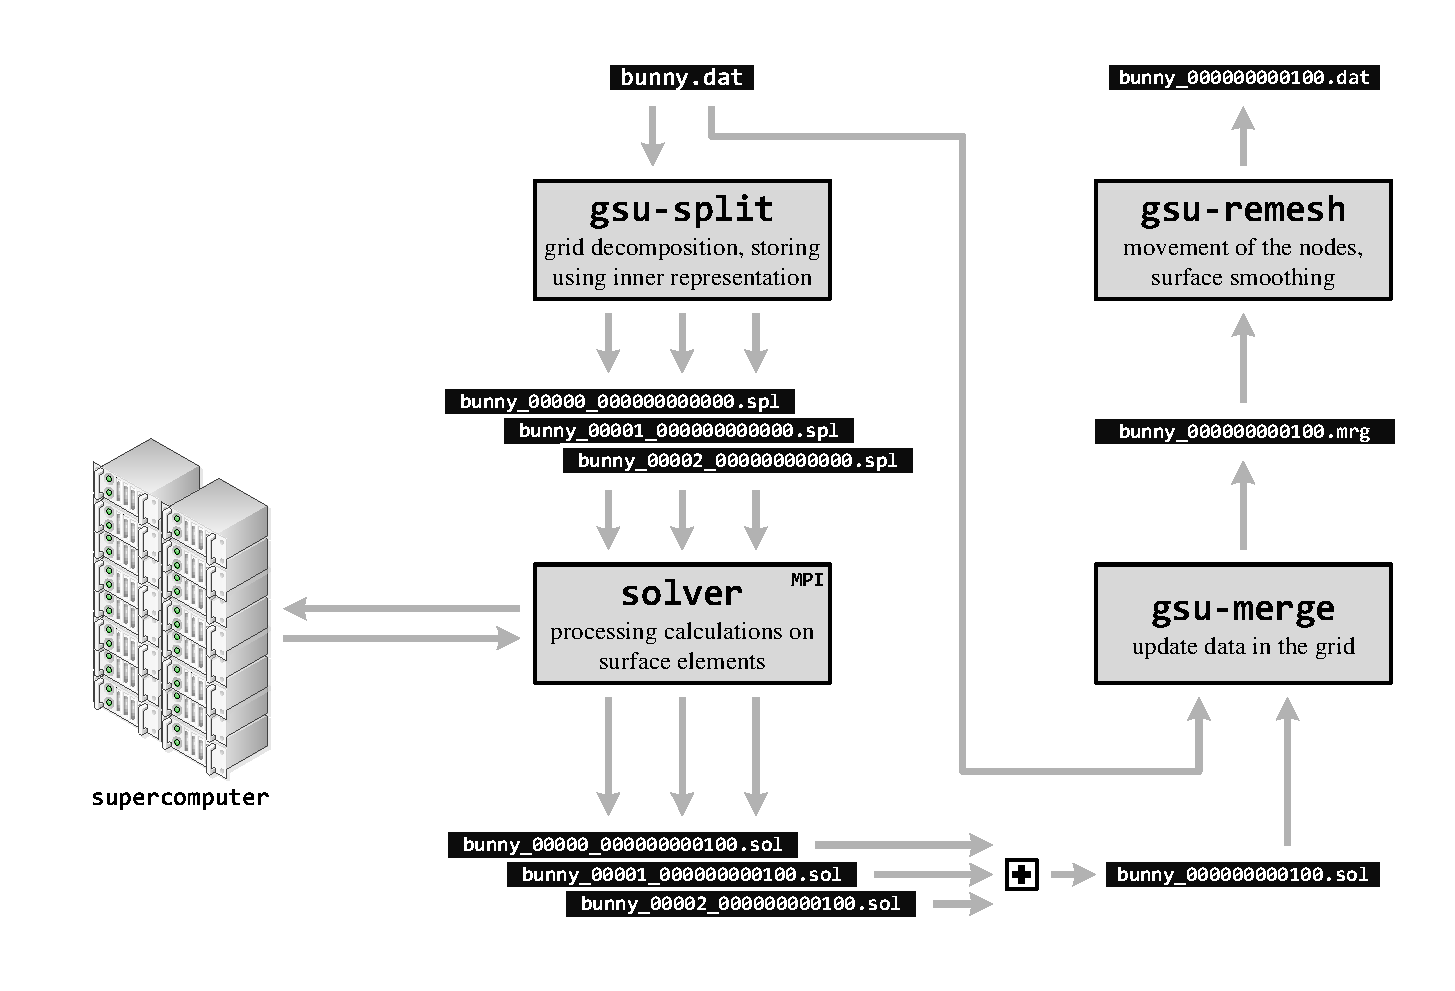
\includegraphics[width=1.0\textwidth]{pics/02-scheme.pdf}
\captionstyle{center}\caption{Схема распараллеливания вычислений на суперкомпьютере.}\label{fig:02-scheme}
\end{figure}

Программная система crys состоит из трех независимых модулей: crys-swim (модуль расчета обледения), crys-gsu (модуль для работы с расчетной сеткой для вычислений в параллельном режиме, а также для консолидации данных сетки), crys-remesh (модуль перестроения поверхности расчетной сетки). Эти модули обмениваются между собой данными исключительно через файлы, находящиеся на файловой системе.
Можно описать поток расчетных данных между модулями следующим образом:

Исходная входная расчетная сетка (bunny.dat) поступает на вход модулю crys-gsu, в котором выполняется разделение расчетной области на отдельные части для обработки в параллельном режиме с помощью MPI. Имя исходной входной расчетной сетки допускается задавать с меткой времени. Если метка времени нулевая, то ее можно опустить, а можно задавать в виде последовательности из 12 нулей (bunny000000000000.dat).
Модуль crys-gsu сохраняет части декомпозированной сетки в отдельные файлы с именами <оригинальное имя сетки><номер MPI процесса (5 разрядов)><метка времени в микросекундах (12 разрядов)>.cry (bunn00003000000000000.cry) в специальном текстовом формате.
Модуль crys-swim выполняет расчеты, используя для этого файлы *.cry, и сохраняет результаты расчетов в файлах с названиями <оригинальное имя сетки<номер MPI процесса (5 разрядов)><метка времени в микросекундах (12 разрядов)>.txt (bunny00003000000000100.txt).
После работы модуля crys-swim файлы *.txt с одинаковой меткой времени, но с разными номерами MPI процессов объединяются в один файл с названием <оригинальное имя сетки><метка времени в микросекундах (12 разрядов)>.txt (bunny000000000100.txt) (данный пункт является опциональным).
Модуль crys-gsu принимает на вход оригинальную расчетную сетку (bunny.dat), а также рассчитанные данные на определенный момент времени (bunny000000000100.txt) и добавляет эти данные к сетке, сохраняя ее под названием <оригинальное имя сетки>r<метка времени в микросекундах (12 разрядов)>.dat (bunnyr000000000100.dat). Суффикс r обозначает файл сетки, подготовленный для перестроения поверхности.
Модуль crys-remesh получает на вход расчетную сетку с посчитанными высотами льда с названием <оригинальное имя сетки>r<метка времени в микросекундах (12 разрядов)>.dat (bunnyr000000000100.dat), выполняет перестроение поверхности и сохраняет сетку под названием <оригинальное имя сетки><метка времени в микросекундах (12 разрядов)>.dat (bunny000000000100.dat)

\section{Декомпозиция неструктурированной расчетной сетки}

\begin{figure}[h]
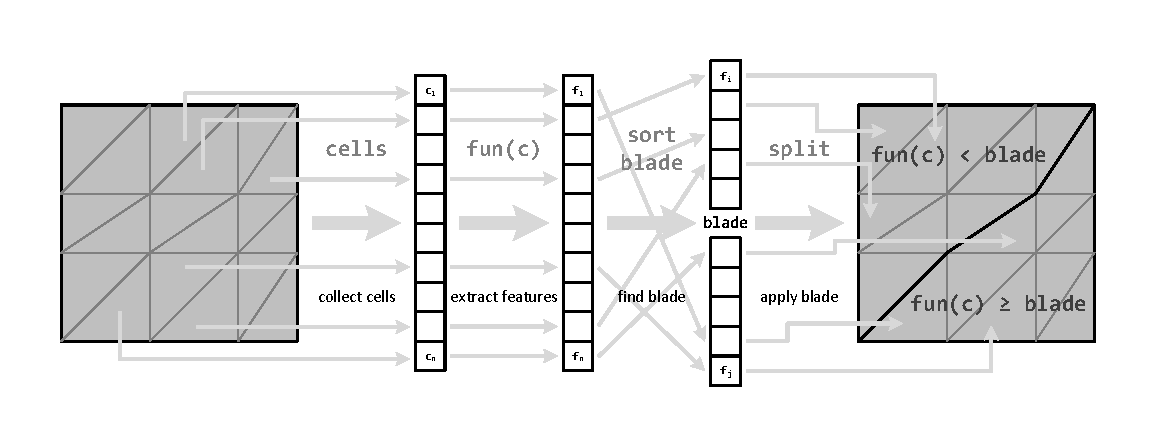
\includegraphics[width=1.0\textwidth]{pics/03-split.pdf}
\captionstyle{center}\caption{Схема разделения домена пополам по выбранному признаку fun.}\label{fig:03-split}
\end{figure}

В работе [22] описан параллельный алгоритм геометрической декомпозиции сеточных данных. Во время работы данного алгоритма происходит последовательное деление текущего домена пополам с помощью сечения плоскостью. На рис. 6. продемонстрирована схема, по которой изначальный головной домен h делится на пару доменов hl (left), hr (right), каждый из которых делится далее пополам и так далее на любое количество доменов, равное степени двойки.

Данный алгоритм предлагается расширить, введя в него произвольные критерии разбиения текущего домена на пару более мелких доменов. Вначале рассмотрим схему простого деления домена пополам с использованием произвольного признака, по которому производится деление (см. рис. 7).

Будем описывать алгоритм разделения домена на две части в нотации языка Python. Пусть задан массив ячеек домена (h  head) и произвольная функция извлечения признака из ячейки (fun). Первым шагом является вычисление массива признаков для всех ячеек (s  signs): s = list(map(fun, h)). После получения массива признаков его нужно отсортировать: s.sort(). В отсортированном массиве признаков следует выбрать среднее значение (b  blade): b = s[len(s) // 2]. Данное значение будет использоваться для разделения домена на два мелких домена (hl  head left, hr  head right) с помощью применения двух простых фильтров: hl, hr = list(filter(h, lambda x: fun(x) < b)), list(filter(h, lambda x: fun(x) >= b)).
После разделения домена на два более мелких домена можно вычислить параметр, отражающий эффективность разбиения. В качестве такого параметра предлагается использовать длину границы между двумя образованными новыми доменами. Таким образом, критерий разбиения зависит от функции вычисления признака (fun). В свою очередь это означает, что при выполнении разбиения не обязательно ограничиваться одной функцией вычисления признака, вместо этого можно подать список функций, для каждой функции вычислитель показатель качества разбиения и в результате остановиться на той функции вычисления признака, которая в конечном итоге приводит к наиболее эффективному разбиению. Если в качестве функций вычисления признака ячейки использовать просто извлечение трех координат центров ячеек, то мы получим в чистом виде алгоритм геометрической декомпозиции сетки с выбором для дробления наиболее протяженного размера по одной из координат. Результат применения данного алгоритма показан на рис. 8

Варьируя набор функций вычисления признаков, по которым можно выполнять разбиение домена, возможно выполнять геометрическую декомпозицию вдоль направления любой кривой, для которой вычисляется проекция ячейки. Декомпозиция с помощью данного метода не ограничивается только геометрическими признаками. Функции вычисления признаков могут использоваться для анализа физических данных ячеек, например, для локализации и выделении в отдельные домены областей с повышенным давлением.
В рамках данной работы описанный алгоритм декомпозиции поверхностной неструктурированной расчетной сетки применялся к поверхностным сеткам, используемым для расчета обледенения поверхности летательного аппарата [24,25]. При расчете обледенения летательного аппарата основной объем вычислений относится к обработке поверхностных ячеек, общие данные между соседними доменами собраны на междоменных ребрах, что обеспечивает небольшой обмен данных, которыми требуется обмениваться в ходе синхронизации вычислений.  Характерный размер таких сеток составил около 105 ячеек, рассматривались как односвязные, так и многосвязные поверхности, а также поверхности, состоящие из нескольких изолированных друг от друга зон.


\begin{figure}[h]
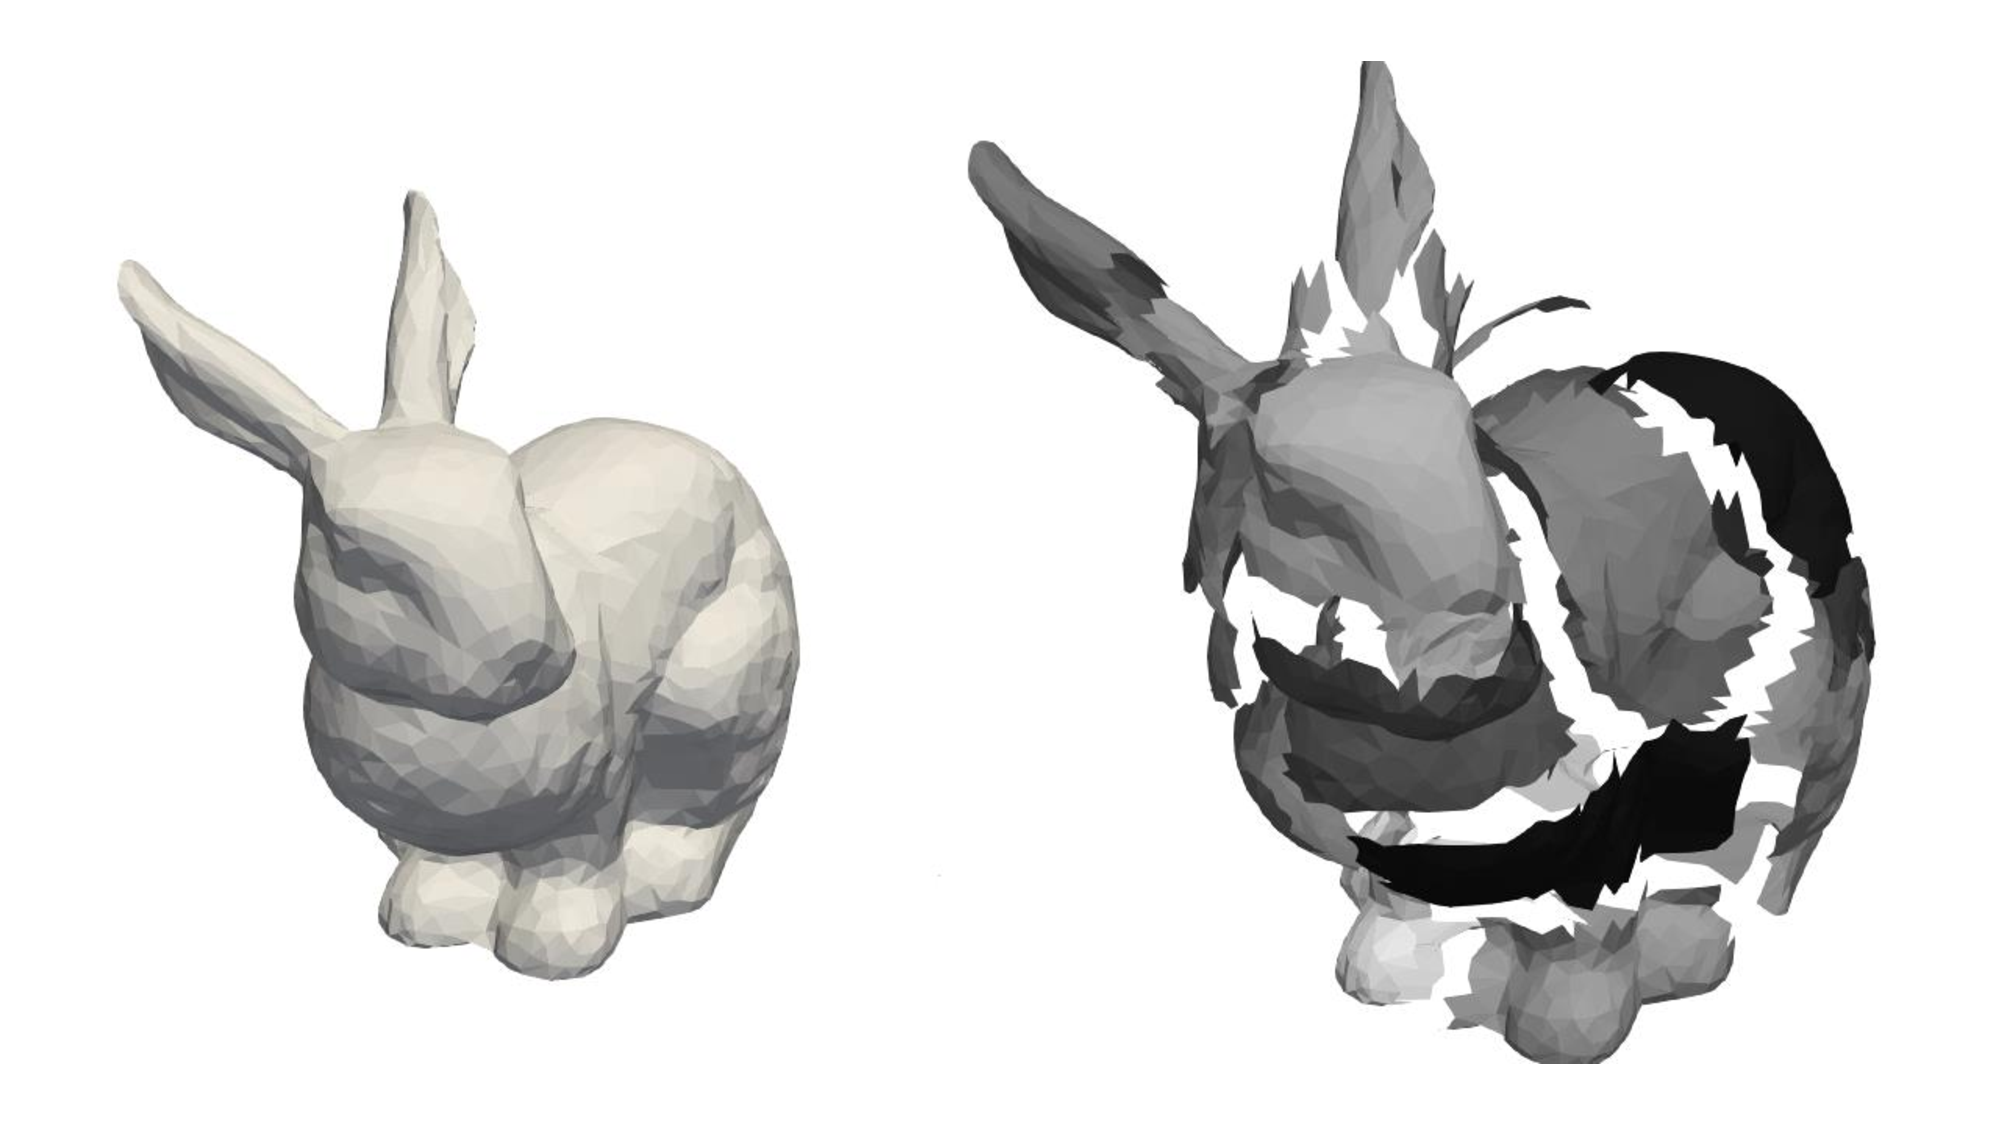
\includegraphics[width=1.0\textwidth]{pics/03-explode-bunny.pdf}
\captionstyle{center}\caption{expand bunny.}\label{fig:03-explode-bunny}
\end{figure}

TODO: Результаты применения hierarchical для тестовых сеток.

\begin{figure}[h]
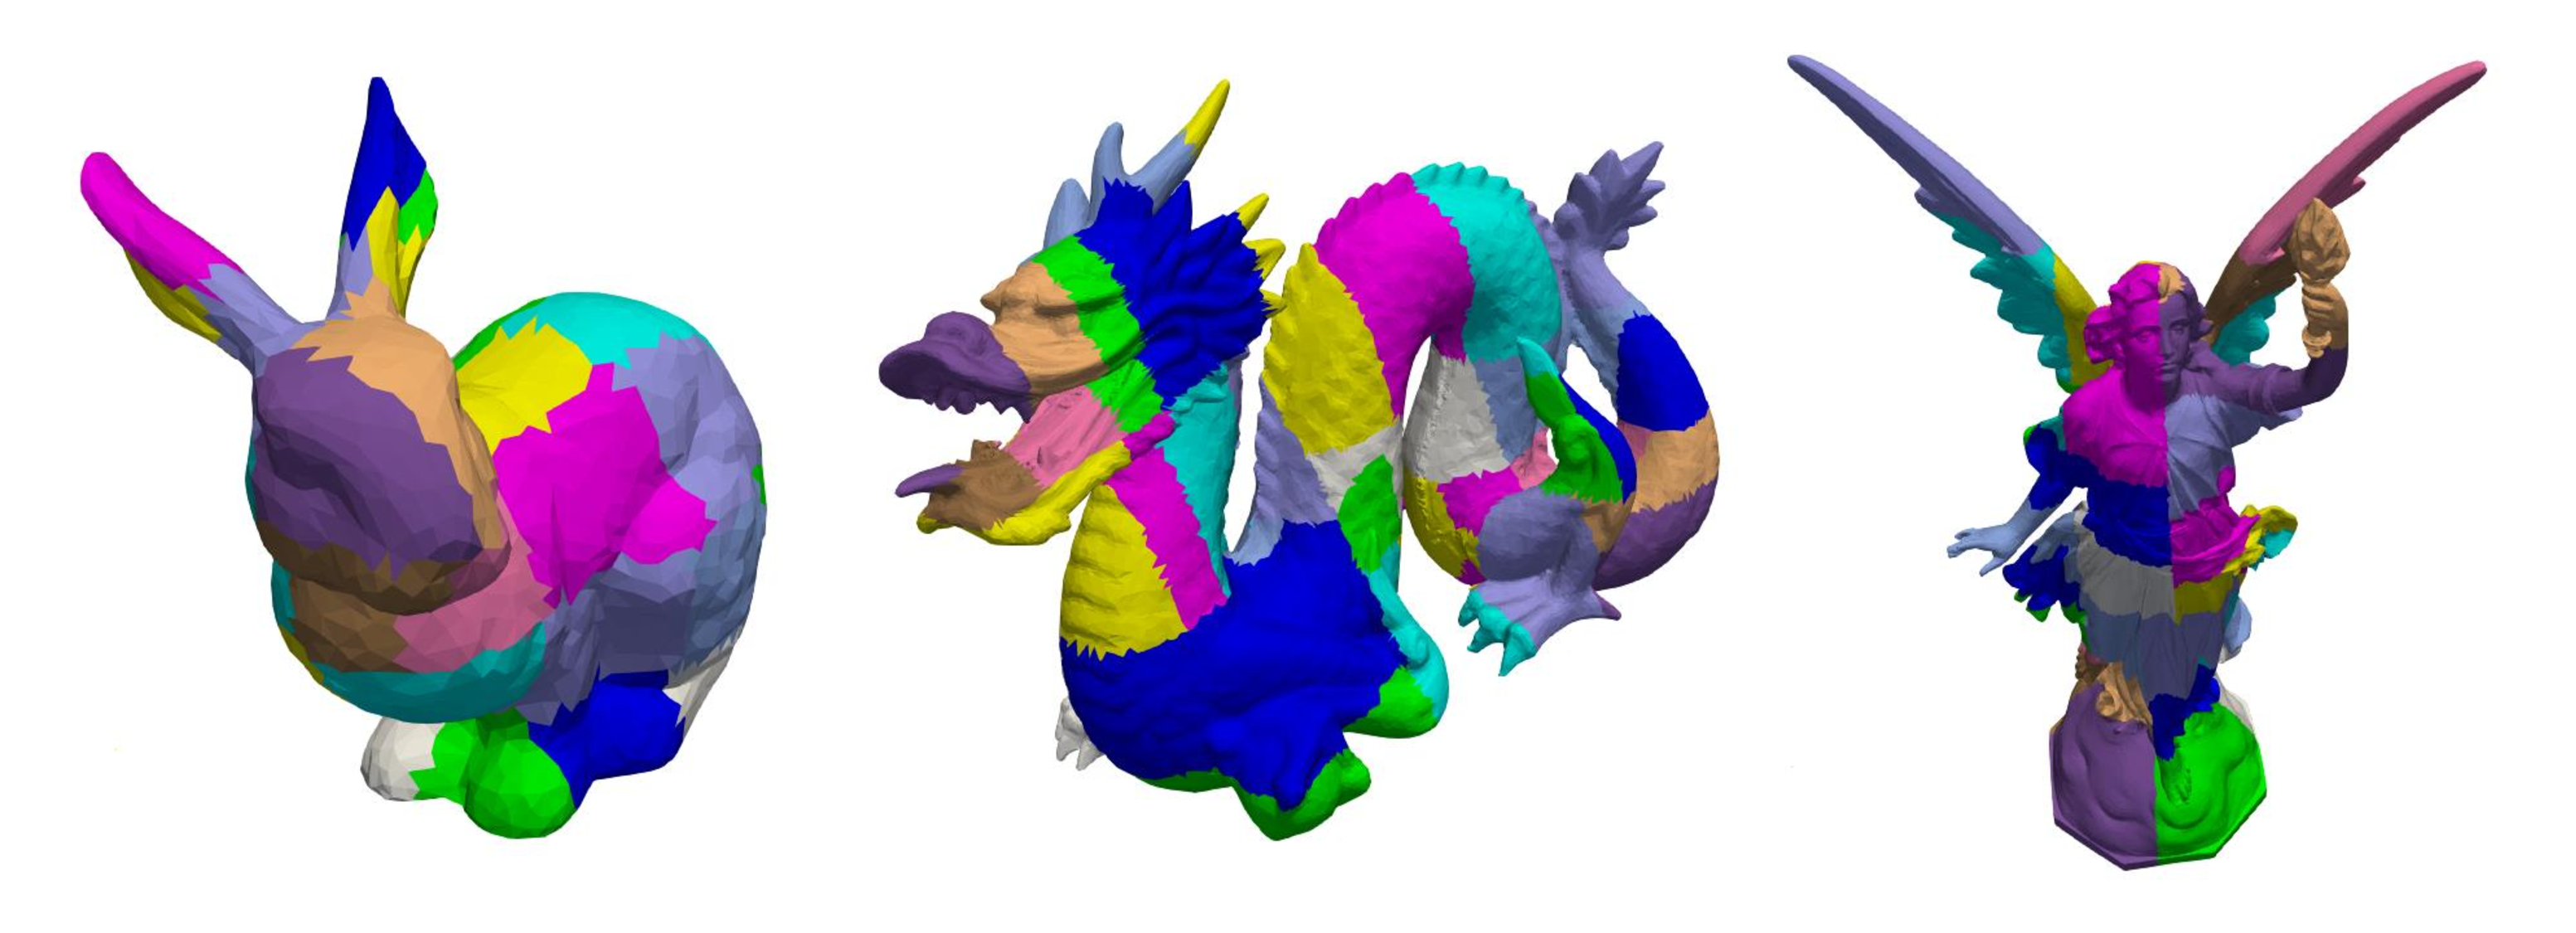
\includegraphics[width=1.0\textwidth]{pics/03-hierarch.pdf}
\captionstyle{center}\caption{hierarch.}\label{fig:03-hierarch}
\end{figure}

TODO

\section{Организация межпроцессных обменов}

\begin{figure}[h]
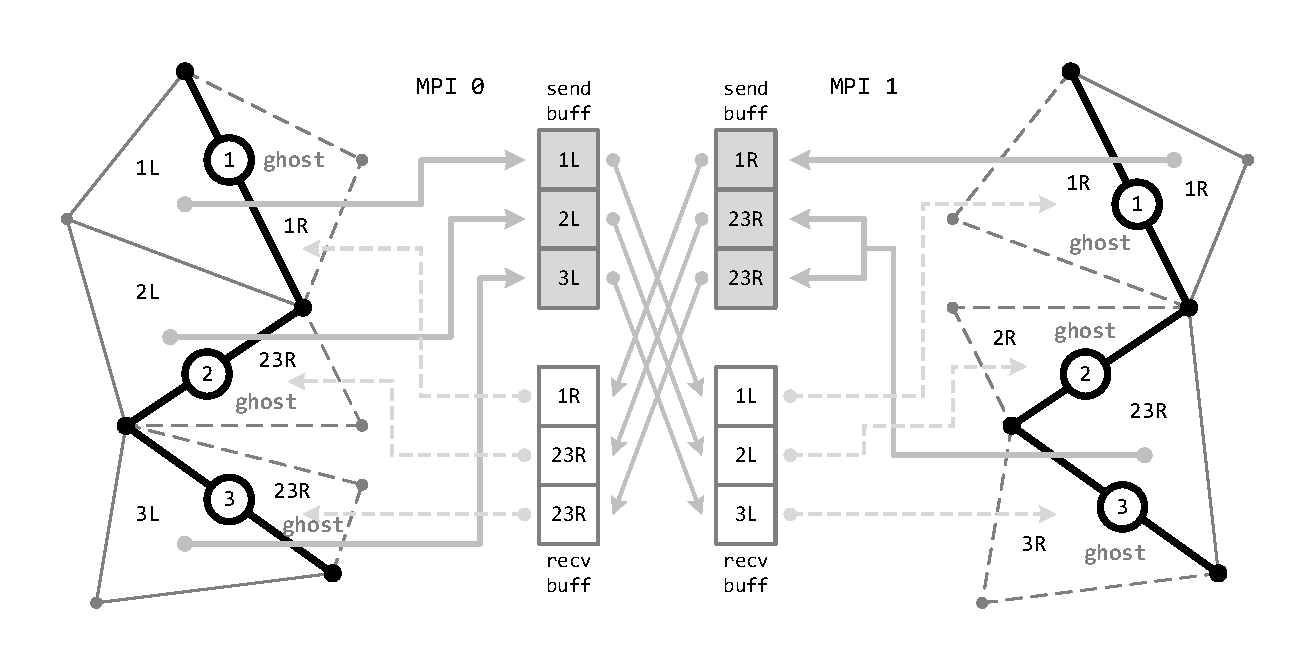
\includegraphics[width=1.0\textwidth]{pics/04-MPI.pdf}
\captionstyle{center}\caption{Схема выполнения MPI-обменов через границу двух зон.}\label{fig:04-MPI}
\end{figure}

TODO описание межпроцессных обменов.

Программа crys-swim должна поддерживать возможность выполнения на кластере на нескольких узлах при этом необходимо обеспечить обмен данными, осуществляемый через границу дробления сетки.
 EI.II.MPI.01. Должна быть поддержана возможность обмена данными между процессами через границу, имеющую произвольную концигурацию. Пример разделения расчетной сетки на две зона (каждая из которых расчитывается в своем процессе) приведен на схеме ниже

EI.II.MPI.02. Для осуществления обменов между процессами в каждом процессе для каждого кросс-ребра должна быть создана фиктивная ячейка, предназначенная для приема данных из соседнего процесса.
Для иллюстрации процесса обменов приведена схема ниже, на которой показано, как граница из предыдущего рисунка раскрывается в окружение MPI-обменов.

На данной схеме видна граница, состоящая из 5 кросс-ребер (0-4, 1-5, 1-6, 2-6, 3-7). При разделении расчетной сетки между двумя процессами в каждом MPI процессе создается по 5 фиктивных ячеек (ghost cells).
 EI.II.MPI.03. Внутри каждого процесса для каждой границы должно быть создано 2 буфера (send buffer и recv buffer) для пересылки и приема данных соответсвенно. Длины буфера определеяется длиной границы.
 EI.II.MPI.04. Должна быть определена следующая последовательность осуществления обмена данными (см. схему выше):

 EI.II.MPI.04.01. Внутри каждого процесса данные из граничных ячеек записываются в send buffer в соответствии с позицией кросс-ребра в границе.

 EI.II.MPI.04.02. Внутри каждого процесса инициируются команды асинхнронного приема сообщений в буферы recv buffer.

 EI.II.MPI.04.03. Внутри каждого процесса инициируются команды асинхронной отправки сообщений из буферов send buffer.

 EI.II.MPI.04.04. Выполнение программы блокируется до завершения всех обменов, после чего во всех процессах внутри буферов recv buffer появляются данные.

 EI.II.MPI.04.05. Внутри каждого процесса данные из recv beffer записываются в фиктивные ячейки в соответствии с позицией кросс-ребра в границе.

\section{Эффективность масштабирования вычислений на суперкомпьютере}

\begin{table}[!h]
\label{tbl:supercomputers}
\setcaptionmargin{0mm}
\onelinecaptionsfalse
\captionstyle{flushleft}
\caption{Конфигурации сегментов суперкомпьютера МВС-10П ОП, на которых производились замеры масштабирования вычислений.}
\bigskip
\begin{tabular}{|c|c|c|c|c|}
\hline
\parbox{3.5cm}{\textit{Семейство\\микропроцессоров}} & \parbox{4.0cm}{\textit{Количество\\процессоров / ядер /\\потоков в узле}} & \parbox{3.5cm}{\textit{Частота\\микропроцессора}} & \parbox{3.0cm}{\textit{Объем\\оперативной\\памяти в узле}} & \parbox{2.5cm}{\textit{Поддержка\\AVX-512}} \\
\hline
Xeon Broadwell & 2 / 32 / 64 & 2.6 GHz & 128 GB & no \\
\hline
Xeon Phi KNL & 1 / 72 / 288 & 1.5 GHz & 96 GB & yes \\
\hline
Xeon Skylake & 2 / 36 / 72 & 3.0 GHz & 192 GB & yes \\
\hline
Xeon Cascade Lake & 2 / 48 / 96 & 3.0 GHz & 192 GB & yes \\
\hline
\end{tabular}
\label{tab:supercomputers}
\end{table}   

\begin{figure}[h]
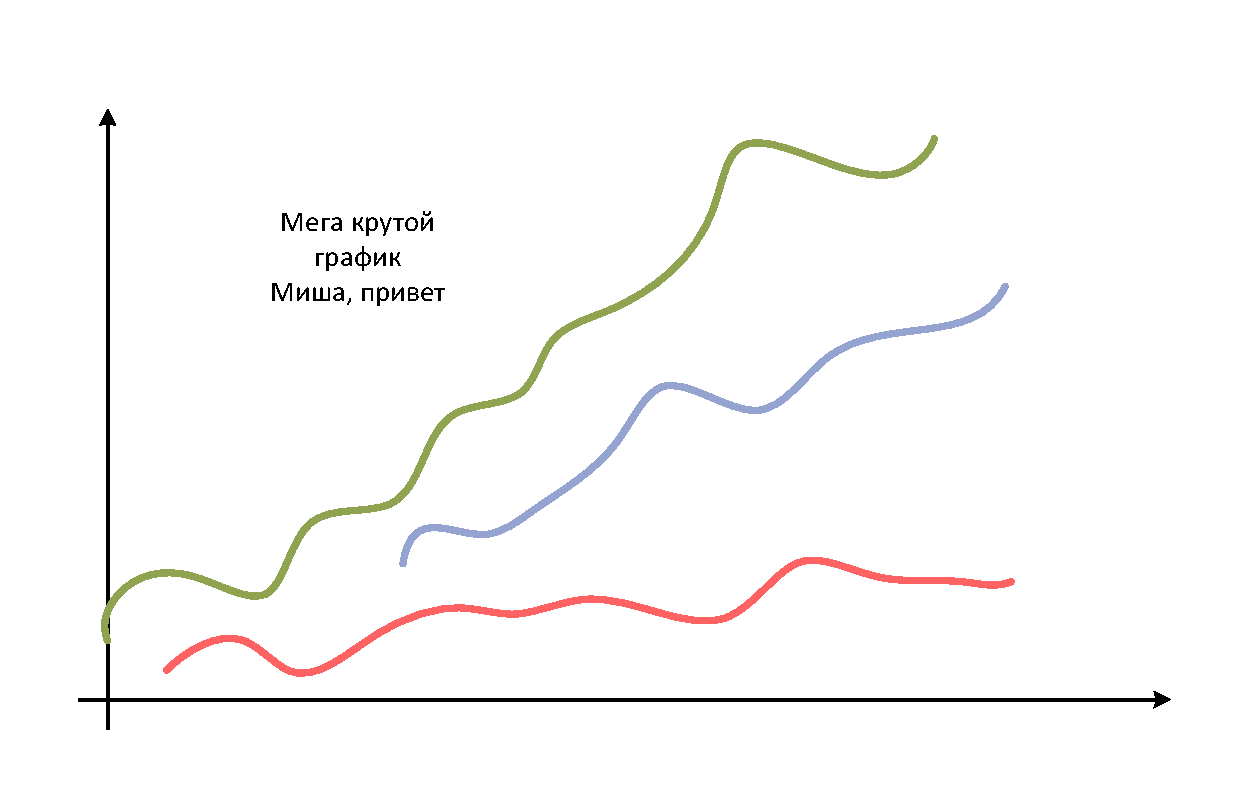
\includegraphics[width=1.0\textwidth]{pics/05-graph.pdf}
\captionstyle{center}\caption{График масшатабируемости вычислений на суперкомпьютерах МСЦ РАН.}\label{fig:05-graph}
\end{figure}

TODO описание запусков

\section{Conclusion}

В ходе выполнения работы рассмотрен ряд алгоритмов декомпозиции поверхностной неструктурированной расчетной сетки и проведен анализ эффективности этих алгоритмов по следующим параметрам: максимальное отклонение размера получившегося домена от идеального значения, доля междоменных ребер в итоговом разбиении, протяженность наиболее длинной границы между доменами. Предложен алгоритм иерархического разбиения доменов расчетной сетки с помощью выбора оптимального критерия разбиения на основе списка функций получения признаков ячеек. Полученные характеристики предложенного алгоритма, простота реализации и скорость его работы позволили использовать данный алгоритм в промышленных программных кодах для декомпозиции поверхностных расчетных сеток с целью улучшения масштабируемости суперкомпьютерных расчетов.

\begin{acknowledgments}
The work has been done at the JSCC RAS as part of the state assignment for the topic 0580-2021-0016.
The supercomputer MVS-10P OP (Broadwell, KNL and Cascade Lake segments), located at the JSCC RAS, was used during the research.
\end{acknowledgments}

\begin{thebibliography}{99}

\bibitem{Rettinger}
\refitem{article}
C. Rettinger, C. Godenschwager, S. Eibl, et al., {\it ``Fully Resolved Simulations of Dune Formation in Riverbeds"}, ISC High Performance , LNCS~{\bf 10266}, 3--21 (2017).

\bibitem{Krappel}
\refitem{article}
T. Krappel, S. Riedelbauch, {\it ``Scale Resolving Flow Simulations of a Francis Turbine Using Highly Parallel CFD Simulations"}, High Performance Computing in Science and Engineering'16, 499--510 (2016).

\bibitem{Markidis}
\refitem{article}
S. Markidis, I. B. Peng, J. L. Tr\"aff, et al.,{\it ``The EPiGRAM Project: Preparing Parallel Programming Models for Exascale"}, ISC High Performance Workshops, LNCS~{\bf 9945}, 56--68  (2016).

\bibitem{Klenk}
\refitem{article}
B.~Klenk, H.~Fr\"oning, {\it ``An Overview of MPI Characteristics of Exascale Proxy Applications"}, ISC High Performance, LNCS~{\bf 10266}, 217--236  (2016).

\bibitem{Abduljabbar}
\refitem{article}
M.~Abduljabbar, G.~S.~Markomanolis, H.~Ibeid, et al., {\it ``An Overview of MPI Characteristics of Exascale Proxy Applications"}, ISC High Performance, LNCS~{\bf 10266}, 79--96 (2017).

\bibitem{Rybakov}
\refitem{article}
A.~A.~Rybakov, {\it ``Inner respresentation and crossprocess exchange mechanism for block-structured grid for supercomputer calculations"}, Program systems: Theory and Application~{\bf 32}(8:1), 121--134 (2017).

\bibitem{Van}
\refitem{article}
R.~F.~Van der Wijngaart, E.~Georganas,~T.~G.~Mattson, et al., {\it ``A New Parallel Research Kernel to Expand Research on Dynamic Load-Balancing Capabilities"}, ISC High Performance, LNCS~{\bf 10266}, 256--274 (2017).

\bibitem{Benderskiy}
\refitem{article}
L.~A.~Benderskiy, D.~A.~Lyubimov, A.~A.~Rybakov, {\it ``Analysis of scaling efficiency in high-speed turbulent flow calculations on a RANS / ILES supercomputer using the high resolution method"}, Trudy SRISA RAS~{\bf 7}(4), 32--40 (2017).

\bibitem{Heller}
\refitem{article}
T.~Heller, H.~Kaiser, P.~Diehl et al., {\it ``Closing the Performance Gap with Modern C++"}, ISC High Performance, LNCS~{\bf 9945}, 18--31 (2016).

\bibitem{Roganov}
\refitem{article}
Roganov V., Osipov V., Matveev G., {\it ``Solving the 2D Poisson PDE by Gauss-Seidel method with parallel programming system"}, Program systems: theory and applications~{\bf 30}(7:3), 99--107 (2016).

% References for REVIEW OF RESEARCH PAPERS section.

\bibitem{Jeffers_KNL}
\refitem{book}
J.~Jeffers, J.~Reinders, A.~Sodani, \emph{Intel Xeon Phi Processor High Performance Programming, Knights Landing Edition} (Morgan Kaufmann, 2016).

\bibitem{Jeffers_KNC}
\refitem{book}
J.~Jeffers, J.~Reinders, \emph{Intel Xeon Phi Coprocessor Processor High Performance Programming} (Morgan Kaufmann, 2013).

\bibitem{Dorris}
\refitem{article}
J.~Dorris, J.~Kurzak , P.~Luszczek, {\it ``Task-Based Cholesky Decomposition on Knights Corner Using OpenMP"}, ISC High Performance, LNCS~{\bf 9945}, 544--562 (2016).

\bibitem{Tobin}
\refitem{article}
J.~Tobin, A.~Breuer, A.~Heinecke et al., {\it ``Accelerating Seismic Simulations Using the Intel Xeon Phi Knights Landing Processor"}, ISC High Performance, LNCS~{\bf 10266}, 139--157 (2017).

\bibitem{McDoniel}
\refitem{article}
W.~McDoniel, M.~Hohnerbach, R.~Canales et al., {\it ``LAMMPS' PPPM Long-Range Solver for the Second Generation Xeon Phi"}, ISC High Performance, LNCS~{\bf 10266}, 61--78 (2017).

\bibitem{Malas}
\refitem{article}
T.~Malas, T.~Kurth, J.~Deslippe, {\it ``Optimization of the Sparse Matrix-Vector Products of an IDR Krylov Iterative Solver in EMGeo for the Intel KNL Manycore Processor"}, ISC High Performance, LNCS~{\bf 9945}, 378--389 (2016).

\bibitem{Krzikalla}
\refitem{article}
O.~Krzikalla, F.~Wende, M.~H\"ohnerbach, {\it ``Dynamic SIMD Vector Lane Scheduling"}, ISC High Performance, LNCS~{\bf 9945}, 354--365 (2016).

\bibitem{Cook}
\refitem{article}
B.~Cook, P.~Maris,M.~Shao, {\it ``High Performance Optimizations for Nuclear Physics Code MFDn on KNL"}, ISC High Performance, LNCS~{\bf 9945}, 366--377 (2016).

\bibitem{Rybakov_Optimization}
\refitem{article}
A.~A.~Rybakov,{\it ``Optimization of the problem of conflict detection with dangerous aircraft movement areas to execute on Intel Xeon Phi"}, Programmnye produkty i sistemy [Software \& Systems]~{\bf 30}(3), 524--528 (2017).

\bibitem{Sengupta}
\refitem{article}
D.~Sengupta,~Y.~Wang,~N.~Sundaram et al., {\it ``Performance Incremental SVM Learning on Intel Xeon Phi Processors"}, ISC High Performance, LNCS~{\bf 10266}, 120--138 (2017).

\bibitem{Kronbichler}
\refitem{article}
M.~Kronbichler,~K.~Kormann ,~I.~Pasichnyk, {\it ``Fast Matrix-Free Discontinuous Galerkin Kernels on Modern Computer Architectures"}, ISC High Performance, LNCS~{\bf 10266}, 237--255 (2017).

\bibitem{Doerfler}
\refitem{article}
D.~Doerfler,~J.~Deslippe ,~S.~Williams, {\it `Applying the Roofline Performance Model to the Intel Xeon Phi Knights Landing Processor"}, ISC High Performance, LNCS~{\bf 9945}, 339--353 (2016).

\bibitem{Rosales}
\refitem{article}
C.~Rosales, J.~Cazes, K.~Milfeld, {\it ``Comparative Study of Application Performance and Scalability on the Intel Knights Landing Processor"}, ISC High Performance, LNCS~{\bf 9945}, 307--318 (2016).

% References for FLAT CYCLES section.

\bibitem{Intel_SDM}
\refitem{manual}
Intel 64 and IA-32 Architectures Software Developer's Manual, Combined Volumes: 1, 2A, 2B, 2C, 2D, 3A, 3B, 3C, 3D and 4, Intel Corporation (2017).

\bibitem{Intel_C}
\refitem{manual}
Intel C++ Compiler 16.0 User and Reference Guide, Intel Corporation (2016).

\bibitem{Intel_Intr}
\refitem{misc}
Intel Intrinsics Guide. \url{https://software.intel.com/sites/landingpage/IntrinsicsGuide/}. Accessed 2018.

\bibitem{Scott_Predct}
\refitem{article}
S.~A.~Mahlke, D.~C.~Lin, W.~Y.~Chen, R.~E.~Hank, {\it ``Effective Compiler Support for Predicated Execution Using the Hyperblock"}, Proceedings of the 25th International Symposium on Microarchitecture, ~45--54 (1992).

\bibitem{Hwu_Predct}
\refitem{article}
W.~W.~Hwu, {\it ``The Superblock: an Effective Technique for VLIW and Superscalar Compilation"}, The Journal of Supercomputing~{\bf 7}(1/2), ~229--248 (1993).

\bibitem{Golub}
\refitem{book}
G.~H.~Golub, C.~F.~Van Loan, {\it ``Matrix Computations"}, (The John Hopkins University Press, 1989).

\bibitem{Zhang}
\refitem{article}
H.~Zhang, R.~T.~Mills, K.~Rupp, B.~F.~Smith, {\it ``Vectorized Parallel Sparse Matrix-Vector Multiplication in PETSc Using AVX-512"}, Proceedings of the 47th International Conference on Parallel Processing (ICPP 2018), ACM, Article 55, 10 pages (2018).

\bibitem{Lyub_RANS_ILES}
\refitem{article}
D.~A.~Lyubimov, {\it ``Development and Application of a High-Resolution Technique for Jet Flow Computation Using Large Eddy Simulation"}, High Temperature~{\bf 50}(3),~420--436 (2012).

\bibitem{Ben_Lyub_Chest_RANS_ILES}
\refitem{article}
L.~A.~Benderskii, D.~A.~Lyubimov, A.~O.~Chestnykh, B.~M.~Shabanov and A.~A.~Rybakov, {\it ``The Use of the RANS/ILES Method to Study the Influence of Coflow Wind on the Flow in a Hot, Nonisobaric, Supersonic Airdrome Jet during Its Interaction with the Jet Blast Deflector"}, High Temperature~{\bf 56}(2),~247--254 (2018).

\bibitem{Aleen}
\refitem{article}
F.~Aleen, V.~P.~Zakharin, R.~Krishnaiyer, G.~Gupta, D.~Kreitzer, C.-S.~Lin, {\it ``Automated Compiler Optimization of Multiple Vector Loads/Stores"}, International Journal of Parallel Programming~{\bf 46}(2),~471--503 (2018).

% References for IRREGULAR ITERATIONS LOOPS section.

\bibitem{Fast_Sort}
\refitem{article}
B.~Bramas, {\it ``Fast Sorting Algorithms Using AVX-512 on Intel Knights Landing"}, arXiv: 1704.08579, Accessed 2018.

\bibitem{Quick_Sort}
\refitem{article}
S.~Gueron, V.~Krasnov, {\it ``Fast Quicksort Implementation Using AVX Instructions"}, The Computer Journal,~{\bf 59}(1),~83--90 (2016).

\bibitem{Quick_Sort_2}
\refitem{article}
B.~Bramas, {\it ``A Novel Hybrid Quicksort Algorithm Vectorized Using AVX-512 on Intel Skylake"}, International Journal of Advanced Computer Science and Applications (IJACSA)~{\bf 8}(10), (2017).

\bibitem{Knuth}
\refitem{book}
D.~E.~Knuth, {\it ``The Art of Computer Programming: Volume 3: Sorting and Searching (2nd Edition)"}, (Addison-Wesley Professional, 1998).

% References for PHYSICAL CALCULATIONS section.

\bibitem{Toro}
\refitem{book}
E.~F.~Toro, {\it ``Riemann Solvers and Numerical Methods for Fluid Dynamics:
A Practical Introduction, 2nd Edition"}, (Springer,1999).

\bibitem{Numerica}
\refitem{misc}
NUMERICA, A Library of Sources for Teaching, Research and Applications, by E.~F.~Toro. \url{https://github.com/dasikasunder/NUMERICA}. Accessed 2018.

\end{thebibliography}

\end{document}
